\documentclass{article}
\usepackage{mathtools}
\usepackage{amsmath}
\usepackage{amssymb}
\usepackage{amsfonts}
\usepackage{graphicx}
\usepackage{float}
\usepackage{multirow}
\usepackage{verbatim}

\linespread{1.3}
\setlength{\parindent}{0em}
\setlength{\parskip}{1em}
\setcounter{secnumdepth}{0}
\setcounter{MaxMatrixCols}{20}
\renewcommand{\arraystretch}{1.5}

\newcommand{\ts}{\textsuperscript}
\newcommand{\diff}{\mathop{}\!\mathrm{d}}
\newcommand{\prob}{\mathbb{P}}
\newcommand{\expect}{\mathbb{E}}
\newcommand{\var}{\text{Var}}

\DeclarePairedDelimiter{\abs}{\lvert}{\rvert}
\DeclarePairedDelimiter\norm{\lVert}{\rVert}
\DeclarePairedDelimiter\p{\lparan}{\rparan}

\title{Assignment 2}
\author{Joshua Hwang (44302650)}

\begin{document}
\section{Exercise 1}
\subsection{a}
Since all are independent (not identical) we can make use of the fact that the
PDF of the vector $Z$ is a product of normal distributions.
\begin{align*}
    f(z) &= \prod_{i=1}^{n+m} g_i (z_i) \\
    &= \prod_{i=1}^m g_x (x_i) \times \prod_{i=1}^n g_y (y_i) \\
\end{align*}

Since the first $m$ elements are iid based on $X$ and the remaining $n$ elements
are iid taken from $Y$ we can cleanly split up our PDF\@. The $g_x$ and $g_y$
respectively are,
\begin{align*}
    g_x(x) &= \frac{1}{\sqrt{2\pi\sigma^2}} e^{-\frac{{(x-\mu_1)}^2}{2\sigma^2}} \\
    g_y (x) &= \frac{1}{\sqrt{2\pi\sigma^2}} e^{-\frac{{(x-\mu_2)}^2}{2\sigma^2}} \\
\end{align*}

We sub these into the previous equation.
\begin{align*}
    L(\sigma, \mu_1, \mu_2;x) &= \prod_{i=1}^m g_x (x_i) \times \prod_{i=1}^n g_y (y_i) \\
    &= \prod_{i=1}^m \frac{1}{\sqrt{2\pi\sigma^2}} e^{-\frac{{(x_i-\mu_1)}^2}{2\sigma^2}}
    \times \prod_{i=1}^n \frac{1}{\sqrt{2\pi\sigma^2}} e^{-\frac{{(y_i-\mu_2)}^2}{2\sigma^2}} \\
    &= {\left(\frac{1}{\sqrt{2\pi\sigma^2}}\right)}^{m+n}
    \prod_{i=1}^m e^{-\frac{{(x_i-\mu_1)}^2}{2\sigma^2}}
    \times \prod_{i=1}^n e^{-\frac{{(y_i-\mu_2)}^2}{2\sigma^2}} \\
    &= {\left(\frac{1}{\sqrt{2\pi\sigma^2}}\right)}^{m+n}
    e^{-\left(\sum_{i=1}^m \frac{{(x_i-\mu_1)}^2}{2\sigma^2}\right)}
    \times e^{-\left(\sum_{i=1}^n \frac{{(y_i-\mu_2)}^2}{2\sigma^2}\right)} \\
    &= {\left(\frac{1}{\sqrt{2\pi\sigma^2}}\right)}^{m+n}
    e^{-\left(\sum_{i=1}^m \frac{{(x_i-\mu_1)}^2}{2\sigma^2}
    + \sum_{i=1}^n \frac{{(y_i-\mu_2)}^2}{2\sigma^2}\right)} \\
    &= {\left(\frac{1}{\sqrt{2\pi\sigma^2}}\right)}^{m+n}
    e^{-\left(\frac{{\sum_{i=1}^m (x_i-\mu_1)}^2 + {\sum_{i=1}^n (y_i-\mu_2)}^2}
    {2\sigma^2}\right)} \\
\end{align*}

The log likelihood is $\ln L(\sigma, \mu_1, \mu_2;x)$.
\begin{align*}
    \ln L(\sigma, \mu_1, \mu_2;x) &= \ln \left({{\left(\frac{1}{\sqrt{2\pi\sigma^2}}\right)}^{m+n}
    e^{-\left(\frac{\sum_{i=1}^m {(x_i-\mu_1)}^2 + \sum_{i=1}^n {(y_i-\mu_2)}^2}
    {2\sigma^2}\right)}}\right) \\
    &= -\left(\frac{m+n}{2}\right) \ln\left(2\pi\sigma^2\right)
    -\left(\frac{\sum_{i=1}^m {(x_i-\mu_1)}^2 + \sum_{i=1}^n {(y_i-\mu_2)}^2}
    {2\sigma^2}\right) \\
\end{align*}

\subsection{b and c}
First find ML estimate for $\sigma$. We will use the log-likelihood.
\begin{align*}
    \ln L(\sigma, \mu_1, \mu_2;x) &= -\left(\frac{m+n}{2}\right) \ln\left(2\pi\sigma^2\right)
    -\left(\frac{\sum_{i=1}^m {(x_i-\mu_1)}^2 + \sum_{i=1}^n {(y_i-\mu_2)}^2}
    {2\sigma^2}\right) \\
    \frac{\partial \ln L(\sigma, \mu_1, \mu_2;x)}{\partial \sigma}
    &= -\left(\frac{m+n}{2}\right) \times \frac{2}{\sigma}
    + \left(\sum_{i=1}^m {(x_i-\mu_1)}^2 + \sum_{i=1}^n {(y_i-\mu_2)}^2\right)
    \frac{2}{2\sigma^3} \\
    &= \left(\sum_{i=1}^m {(x_i-\mu_1)}^2 + \sum_{i=1}^n {(y_i-\mu_2)}^2\right)
    \frac{1}{\sigma^3}
    - \frac{m+n}{\sigma} \\
    \text{Find the maximal point} \\
    0 &= \left(\sum_{i=1}^m {(x_i-\mu_1)}^2 + \sum_{i=1}^n {(y_i-\mu_2)}^2\right)
    \frac{1}{\sigma^3}
    - \frac{m+n}{\sigma} \\
    0 &= \left(\sum_{i=1}^m {(x_i-\mu_1)}^2 + \sum_{i=1}^n {(y_i-\mu_2)}^2\right)
    - {(m+n)}{\sigma^2} \\
    (m+n)\sigma^2 &= \left(\sum_{i=1}^m {(x_i-\mu_1)}^2 + \sum_{i=1}^n {(y_i-\mu_2)}^2\right) \\
    \sigma^2 &= \frac{\sum_{i=1}^m {(x_i-\mu_1)}^2 + \sum_{i=1}^n {(y_i-\mu_2)}^2}{m+n} \\
    \sigma &= \sqrt{\frac{\sum_{i=1}^m {(x_i-\mu_1)}^2 + \sum_{i=1}^n {(y_i-\mu_2)}^2}{m+n}} \\
\end{align*}

Now find for $\mu_1$ and $\mu_2$.
\begin{align*}
    \ln L(\sigma, \mu_1, \mu_2;x) &= -\left(\frac{m+n}{2}\right) \ln\left(2\pi\sigma^2\right)
    -\left(\frac{\sum_{i=1}^m {(x_i-\mu_1)}^2 + \sum_{i=1}^n {(y_i-\mu_2)}^2}
    {2\sigma^2}\right) \\
    \ln f(z) &= -\left(\frac{m+n}{2}\right) \ln\left(2\pi\sigma^2\right)
    -\left(\frac{\sum_{i=1}^m {(x_i^2-2x_i\mu_1 + \mu_1^2)}
    + \sum_{i=1}^n {(y_i^2-2y_i\mu_2+\mu_2^2)}}
    {2\sigma^2}\right) \\
    \frac{\partial\ln f(z)}{\partial \mu_1}
    &= -\left(\frac{\sum_{i=1}^m {(2\mu_1 - 2x_i)}}
    {2\sigma^2}\right) \\
    &= \left(\frac{\sum_{i=1}^m {(x_i - \mu_1)}}
    {\sigma^2}\right) \\
    &= \left(\frac{\sum_{i=1}^m x_i - \sum_{i=1}^m\mu_1}
    {\sigma^2}\right) \\
    &= \left(\frac{\sum_{i=1}^m x_i - m\mu_1}
    {\sigma^2}\right) \\
    &= \frac{\sum_{i=1}^m x_i}{\sigma^2} - \frac{m\mu_1}{\sigma^2} \\
    \text{Find the maximal point} \\
    0 &= \frac{\sum_{i=1}^m x_i}{\sigma^2} - \frac{m\mu_1}{\sigma^2} \\
    \mu_1 &= \frac{\sum_{i=1}^m x_i}{m} \\
\end{align*}

The process is repeated for the $\mu_2$ but it's the exact same process so we'll
just state the result.
\begin{align*}
    \mu_2 &= \frac{\sum_{i=1}^n y_i}{n} \\
\end{align*}

\subsection{d}
The ML estimate for $(\mu_1, \mu_2, \sigma^2)$ is,
\begin{align*}
    T(z) &= \left(\frac{\sum_{i=1}^m x_i}{m},\frac{\sum_{i=1}^n y_i}{n},
    \frac{\sum_{i=1}^m {(x_i-\mu_1)}^2 + \sum_{i=1}^n {(y_i-\mu_2)}^2}{m+n}\right)
\end{align*}

and the estimator is,
\begin{align*}
    T(Z) &= \left(\frac{\sum_{i=1}^m X_i}{m},\frac{\sum_{i=1}^n Y_i}{n},
    \frac{\sum_{i=1}^m {(X_i-\mu_1)}^2 + \sum_{i=1}^n {(Y_i-\mu_2)}^2}{m+n}\right)
\end{align*}

\subsection{e}
Since all $A_i$ are iid and normally distributed with unknown $\mu \geq 0$ we
can take the product of the pdf and the realised vector of $A$s.
\begin{align*}
    L(\mu;x) &= \prod_{i=1}^n g_a (a_i) \\
    &= \prod_{i=1}^n \frac{1}{\sqrt{2\pi\sigma^2}} e^{-\frac{{(a_i-\mu)}^2}{2\sigma^2}} \\
    &= \prod_{i=1}^n \frac{1}{\sqrt{2\pi}} e^{-\frac{{(a_i-\mu)}^2}{2}} \\
\end{align*}

We then take the log likelihood and it's derivative.
\begin{align*}
    \ln L(\mu;x) &= \ln \prod_{i=1}^n \frac{1}{\sqrt{2\pi}} e^{-\frac{{(a_i-\mu)}^2}{2}} \\
    &= -\frac{n}{2} \ln(2\pi) - \sum_{i=1}^n \frac{{(a_i-\mu)}^2}{2} \\
    \frac{\partial \ln L(\mu;x)}{\partial \mu}
    &= - \sum_{i=1}^n \frac{2\mu - 2a_i}{2} \\
    &= \sum_{i=1}^n a_i - n\mu \\
    \text{Find the maximal point} \\
    0 &= \sum_{i=1}^n a_i - n\mu \\
    \mu &= \frac{\sum_{i=1}^n a_i}{n} \\
\end{align*}

We must recall that $\mu \geq 0$. Thus if our realisation is negative the most
likely and \textbf{possible} scenario for $\mu$ must be $\mu = 0$.

The ML estimator $(\mu)$ for this distribution is,
\begin{align*}
    T(A)
    &=
    \begin{cases}
        \frac{\sum_{i=1}^n A_i}{n} &\text{if it's non-negative} \\
        0 &\text{otherwise}
    \end{cases}
\end{align*}

\section{Exercise 2}
\subsection{a}
A PDF must integrate to 1 and must never be negative.
Through observation we see that given $\lambda > 0$ our PDF will never be
negative.
\begin{align*}
    \int_{-\infty}^\infty g_\lambda(y)
    \times I_{y \in [\lambda, \infty)} \diff y
    &= \int_\lambda^\infty \lambda y^{-2} \diff y \\
    &= \lambda \int_\lambda^\infty y^{-2} \diff y \\
    &= -\lambda \left(\frac{1}{\infty} - \frac{1}{\lambda}\right) \\
    &= 1 \\
\end{align*}

Thus it is a PDF\@.

\subsection{b}
Since $X_i$ are iid we can take the product to get the joint PDF\@.
\begin{align*}
    L(\lambda;x) &= \prod_{i=1}^n g_\lambda (x_i) \\
    &= \prod_{i=1}^n \lambda x_i^{-2} \times I_{x_i \in [\lambda, \infty)} \\
    &= \lambda^n \prod_{i=1}^n x_i^{-2} \times I_{x_i \in [\lambda, \infty)} \\
\end{align*}

\subsection{c}
We cannot differentiate since our PDF is piecewise and not smooth.
Instead we appeal to intuition. Our maximum can only be achieved by ensuring all
points are within $[\lambda, \infty)$. Not only but as $\lambda$ increases the
likelihood increases. Thus the maximal choice for $\lambda$ is the minimum of
$(x_1, x_2, \ldots, x_n)$. 
\begin{align*}
    T(x) &= \min (x_1, x_2, \ldots, x_n)
\end{align*}

Additionally,
\begin{align*}
    T(X) &= \min (X_1, X_2, \ldots, X_n)
\end{align*}

\subsection{d}
\begin{align*}
    \prob_\lambda (T(X) > y) &= \prob_\lambda (\min (X_1, X_2, \ldots, X_n) > y) \\
\end{align*}

This is only true then all $X_i > y$. Since all $X_i$ are independent this is
just.
\begin{align*}
    \prob_\lambda (\min (X_1, X_2, \ldots, X_n) > y) &= \prob_\lambda (X > y)^n \\
    &= (1-\prob_\lambda (X \leq y))^n \\
    &= (1-G_\lambda(y))^n \\
\end{align*}

We now need to find $G(X)$ which is just the integral of $g(y)$.
\begin{align*}
    G(x) &= \int_{\lambda}^x g(y) \diff y \\
    &= \int_{\lambda}^x \lambda y^{-2} \diff y \\
    &= \lambda \int_{\lambda}^x y^{-2} \diff y \\
    &= - \lambda \left[ y^{-1} \right]_\lambda^x \\
    &= \lambda \left[ y^{-1} \right]^\lambda_x \\
    &= \lambda \left[ \lambda^{-1} - x^{-1} \right] \\
    &= 1 - \lambda x^{-1} \\
\end{align*}

Now coming back to our previous equation,
\begin{align*}
    \prob_\lambda (\min (X_1, X_2, \ldots, X_n) > y) &= (1-G_\lambda(y))^n \\
    &= (1-(1 - \lambda y^{-1}))^n \\
    &= (\lambda y^{-1})^n \\
    \prob_\lambda (T(X) > y) &= \left(\frac{\lambda}{y}\right)^n \\
\end{align*}

\subsection{e}
A cumulative distribution is defined as $F(x) = \prob (X \leq x)$.
\begin{align*}
    F_\lambda (y) &= \prob_\lambda (T(X) \leq y) \\
    &= 1 - \prob_\lambda (T(X) > y) \\
    &= 1 - \left(\frac{\lambda}{y}\right)^n \\
\end{align*}

\subsection{f}
The PDF given the CDF is derived by differentiating the CDF by $y$.
\begin{align*}
    F_\lambda (y) &= 1 - \left(\frac{\lambda}{y}\right)^n \\
    &= 1 - \frac{\lambda^n}{y^n} \\
    &= 1 - \lambda^n y^{-n} \\
    {F'}_\lambda (y) &= n \lambda^n y^{-n-1} \\
    f_\lambda (y) &= n \lambda^n y^{-n-1} \\
\end{align*}

\subsection{g}
\begin{align*}
    \expect_\lambda(T(X) - \lambda)
    &= \expect_\lambda(T(X)) - \lambda \\
    &= \int_{-\infty}^{\infty} f_\lambda(y) \times y \diff y - \lambda \\
    &= \int_{\lambda}^{\infty} n \lambda^n y^{-n-1} \times y \diff y - \lambda \\
    &= n \lambda^n \int_{\lambda}^{\infty} y^{-n} \diff y - \lambda \\
    &= n \lambda^n \frac{1}{1-n} \left[y^{1-n}\right]_{\lambda}^{\infty} - \lambda \\
    &= \frac{n \lambda^n}{1-n} \left[y^{1-n}\right]_{\lambda}^{\infty} - \lambda \\
    &= \frac{n \lambda^n}{1-n} \left[(1/y)^{n-1}\right]_{\lambda}^{\infty} - \lambda \\
    &= \frac{n \lambda^n}{1-n} \left[0 - (1/\lambda)^{n-1}\right] - \lambda \\
    &= \frac{n \lambda^n}{n-1} (1/\lambda)^{n-1} - \lambda \\
    &= \frac{n \lambda}{n-1} - \lambda \\
    &= \lambda \left(\frac{n}{n-1} - 1\right) \\
    &= \left(\frac{n - (n-1)}{n-1}\right)\lambda  \\
    &= \left(\frac{1}{n-1}\right)\lambda  \\
\end{align*}

\subsection{h}
Mean square error is defined as
\begin{align*}
    MSE(\lambda; T) &= \var_\lambda (T) + \left(\expect_\lambda (T - \lambda)\right)^2 \\
\end{align*}

We already have the $\expect_\lambda (T - \lambda)$
thus all we need is $\var_\lambda (T)$.

\begin{align*}
    \var_\lambda (T) &= \expect(T^2) - (\expect(T))^2 \\
    &= \expect(T^2) - (\expect(T))^2 \\
\end{align*}

We know $\expect(T)$ since we calculated it earlier. We now find $\expect(T^2)$.
\begin{align*}
    \expect(T^2) &= \int_\lambda^\infty f_\lambda(y) \times y^2 \diff y \\
    &= \int_\lambda^\infty n \lambda^n y^{-n-1} \times y^2 \diff y \\
    &= \int_\lambda^\infty n \lambda^n y^{1-n} \diff y \\
    &= n \lambda^n \int_\lambda^\infty y^{1-n} \diff y \\
    &= n \lambda^n \frac{1}{2-n} \left[y^{2-n}\right]_\lambda^\infty \\
    &= n \lambda^n \frac{1}{2-n} \left[(1/y)^{n-2}\right]_\lambda^\infty \\
    &= n \lambda^n \frac{1}{2-n} \left[0 - (1/\lambda)^{n-2}\right] \\
    &= n \lambda^n \frac{1}{n-2} (1/\lambda)^{n-2} \\
    &= n \lambda^2 \frac{1}{n-2} \\
    &= \frac{n \lambda^2}{n-2} \\
\end{align*}

Going back to the $\expect(T^2) - (\expect(T))^2$.
\begin{align*}
    \expect(T^2) - (\expect(T))^2
    &= \frac{n \lambda^2}{n-2} - \left(\frac{n \lambda}{n-1}\right)^2 \\
    &= \frac{n \lambda^2}{n-2} - \frac{n^2 \lambda^2}{(n-1)^2} \\
    &= \frac{n \lambda^2 (n-1)^2}{(n-2)(n-1)^2} - \frac{n^2 \lambda^2 (n-2)}{(n-2)(n-1)^2} \\
    &= \frac{n \lambda^2 (n-1)^2 - n^2 \lambda^2 (n-2)}{(n-2)(n-1)^2} \\
    &= \lambda^2 \frac{n(n-1)^2 - n^2(n-2)}{(n-2)(n-1)^2} \\
    &= \lambda^2 \frac{n}{(n-2)(n-1)^2} \\
    \var_\lambda (T) &= \frac{n\lambda^2}{(n-2)(n-1)^2} \\
\end{align*}

Now back to our original question,
\begin{align*}
    MSE(\lambda; T) &= \var_\lambda (T) + \left(\expect_\lambda (T - \lambda)\right)^2 \\
    &= \frac{n\lambda^2}{(n-2)(n-1)^2} + \left(\left(\frac{1}{n-1}\right)\lambda\right)^2 \\
    &= \frac{n\lambda^2}{(n-2)(n-1)^2} + \left(\frac{1}{(n-1)^2}\right)\lambda^2 \\
    &= \frac{n\lambda^2}{(n-2)(n-1)^2} + \frac{\lambda^2}{(n-1)^2} \\
    &= \frac{n\lambda^2}{(n-2)(n-1)^2} + \frac{\lambda^2(n-2)}{(n-2)(n-1)^2} \\
    &= \frac{n\lambda^2 + \lambda^2(n-2)}{(n-2)(n-1)^2} \\
    &= \frac{\lambda^2(2n-2)}{(n-2)(n-1)^2} \\
    &= \frac{2\lambda^2}{(n-2)(n-1)} \\
\end{align*}

\section{Exercise 3}
\subsection{a}
Observe that for $U_{(n)} \leq u$ we need to ensure that all $U_i \leq u$.
The probability that all $U_i \leq u$ (since all $U_i$ are independent and the
uniforms are between 0 and 1) is given by $u^n$. Of course this only applies
when $u$ is chosen between 0 and 1, if $u$ was chosen outside these bounds then
the random variable $U_{(n)}$ could not possibly reach those values thus.
\begin{align*}
    \prob(U_{(n)} \leq u)
    &=
    \begin{cases}
        0, & u < 0 \\
        u^n, & 0 \leq u \leq 1 \\
        0, & u > 1
    \end{cases}
\end{align*}

\subsection{b}
Note that
\begin{align*}
    \prob(U_{(n)} > u) &= 1 - \prob(U_{(n)} \leq u) \\
\end{align*}

When $u = 0$ then $\prob(U_{(n)} > 0) = 1$. Since all $a$ and $b$ outside the
range of $[0,1]$ are equivalent to those $=0$ or $=1$ we shall just focus on the
$u \in [0,1]$.

\begin{align*}
    \prob(a \leq U_{(n)} \leq b) &= \prob(U_{(n)} \leq b) - \prob(U_{(n)} < a) \\
    &= b^n - a^n \\
    \text{Force to take the probability as 95\%} \\
    0.95 &= b^n - a^n \\
\end{align*}

We now choose an $a$ and $b$ that satisfy this. Choose $b=1$.
\begin{align*}
    0.95 &= b^n - a^n \\
    0.95 &= 1^n - a^n \\
    a &= \sqrt[n]{0.05} \\
\end{align*}

\subsection{c}
The PDF of a single uniform is $\frac{1}{\theta - 0}$. Thus ML for this is
\begin{align*}
    L(\theta; X) &= \prod_{i=1}^n \frac{1}{\theta} \\
    &= \theta^{-n} \\
\end{align*}

We observe that the function is monotone decreasing. Thus the most optimal point
is when $\theta \to 0$. But note that each $U \ngeq \theta$ thus the maximal
likelihood is when $\theta = \max\{X_1, X_2, \ldots, X_n\}$.

\subsection{d}
We note that all $U(a,b) \sim (a-b)U(0,1) + b$. Thus our $U(0, \theta) \sim 
\theta U(0,1)$. Also note that 
$\max\{a,b\}/c = \max\{\frac{a}{c},\frac{b}{c}\}$ when $c$ is positive.
Thus we find,
\begin{align*}
    X_{(n)}/\theta &= \frac{\max\{X_1, X_2, \ldots, X_n\}}{\theta} \\
    &= \frac{\max\{\theta U_1, \theta U_2, \ldots, \theta U_n\}}{\theta} \\
    &= \max\{U_1, U_2, \ldots, U_n\} \\
\end{align*}

Which now no longer depends on $\theta$ thus it is a pivot variable.

\subsection{e}
We make the connection that the MLE of $\theta$ can be taken by using the fact
that $X_{(n)}/\theta = U_{(n)}$ the $U_{(n)}$. We choose the confidence interval
created in part b.
\begin{align*}
    0.95 &= \prob\left(\sqrt[n]{0.05} \leq U_{(n)} \leq 1\right) \\
    0.95 &= \prob\left(\sqrt[n]{0.05} \leq \frac{X_{(n)}}{\theta} \leq 1\right) \\
    0.95 &= \prob\left(\frac{1}{\sqrt[n]{0.05}} \geq \frac{\theta}{X_{(n)}} \geq 1\right) \\
    0.95 &= \prob\left(\frac{X_{(n)}}{\sqrt[n]{0.05}} \geq \theta \geq X_{(n)}\right) \\
    0.95 &= \prob\left(X_{(n)} \leq \theta \leq \frac{X_{(n)}}{\sqrt[n]{0.05}}\right) \\
    \hat{\theta} &\in \left[X_{(n)}, \frac{X_{(n)}}{\sqrt[n]{0.05}}\right] \\
\end{align*}

Our estimate for $\theta$ is given by the maximum of the data, $2.364$. Thus,
\begin{align*}
    \hat{\theta} &\in \left[X_{(n)}, \frac{X_{(n)}}{\sqrt[n]{0.05}}\right] \\
    \hat{\theta} &\in \left[2.364, \frac{2.364}{\sqrt[8]{0.05}}\right] \\
    \hat{\theta} &\in \left[2.364, 3.438\right] \\
\end{align*}

\section{Exercise 4}
\subsection{a}
The block either breaks or it doesn't thus it is a Bernoulli model.
The significance level is the probability that we reject the null hypothesis
despite the null hypothesis being correct.
The set of 50 tests creates a binomial, $X \sim Bin(50,0.4)$.
\begin{align*}
    \alpha &= \prob(X \leq 14 \cup X \geq 26) \\
    &= 1 - \prob(14 < X < 26) \\
    &= 1 - \left(\prob(X < 26) - \prob(X \leq 14)\right) \\
    &= 1 - \left(\prob(X \leq 25) - \prob(X \leq 14)\right) \\
    &= 1 - \left(0.943 - 0.054\right) \\
    &= 1 - 0.889 \\
    &= 0.111 \\
\end{align*}

Thus the significance level is 0.111.

\subsection{b}
The power, $1-\beta$, is the probability that we reject the null hypothesis
knowing that the alternative hypothesis is right. The opposite is of course 
$\beta$ which gives you the probability that we maintain the null hypothesis
despite the fact that the null hypothesis is wrong.
\begin{align*}
    \beta &= \prob(14 < X < 26) \\
    &= \prob(X < 26) - \prob(X \leq 14) \\
    &= \prob(X \leq 25) - \prob(X \leq 14) \\
    &= \prob(X \leq 25) - \prob(X \leq 14) \\
\end{align*}

\begin{verbatim}
----In R----
p = seq(0,1,0.01)
beta = pbinom(25,50,p) - pbinom(14,50,p)
plot(p,beta)
\end{verbatim}

\begin{figure}[h]
    \centering
    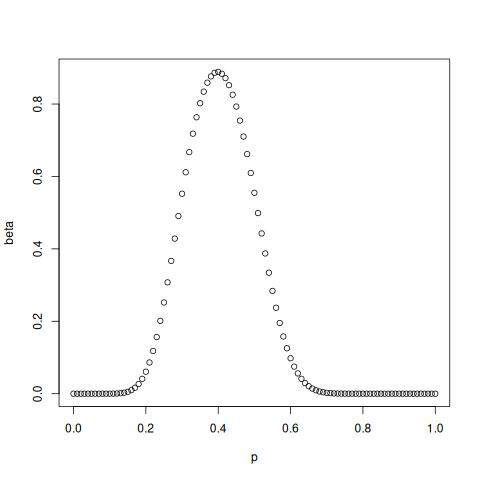
\includegraphics[width=\textwidth]{img/rplot.jpg}
\end{figure}

\subsection{c}
The likelihood ratio test is,
\begin{align*}
    \frac{L(p=0.4;X)}{L(p=0.5;X)}
\end{align*}

The likelihood is given by,
\begin{align*}
    L(p;x) &= {}^{50}C_x p^x (1-p)^{50-x} \\
    L(p=0.4;x) &= {}^{50}C_x 0.4^x 0.6^{50-x} \\
    L(p=0.5;x) &= {}^{50}C_x 0.5^x 0.5^{50-x} \\
    &= {}^{50}C_x 0.5^{50} \\
\end{align*}

Now we return to the other part,
\begin{align*}
    \frac{L(p=0.4;X)}{L(p=0.5;X)}
    &= \frac{{}^{50}C_x 0.4^x 0.6^{50-x}}
    {{}^{50}C_x 0.5^{50}} \\
    &= \frac{0.4^x 0.6^{50-x}}{0.5^{50}} \\
    &= 2^{50} 0.4^x 0.6^{50-x} \\
\end{align*}

\subsection{d}
Given some cutoff $k$,
\begin{align*}
    \frac{L(p=0.4;X)}{L(p=0.5;X)} &\leq k \\
    2^{50} 0.4^x 0.6^{50-x} &\leq k \\
\end{align*}

We claim that this equation lowers as $x$ increases.
Though it may not be obvious currently let's take a look at the derivative.
\begin{align*}
    2^{50} 0.4^x 0.6^{50-x} 
    &\to 2^{50} \ln(0.4) 0.4^x 0.6^{50-x} - 2^{50} 0.4^x \ln(0.6) 0.6^{50-x} \\
    &= 2^{50} (\ln(0.4) - \ln(0.6)) 0.4^x 0.6^{50-x} \\
\end{align*}

Since logarithms are increasing functions we know that $\ln(0.4) < \ln(0.6)$.
Thus we conclude that the derivative is negative. As $x$ increases 
$2^{50} 0.4^x 0.6^{50-x}$ becomes smaller. Thus having a cutoff of $\leq k$ is
equivalent to $\{X \geq c\}$ with some cutoff $c$.

\subsection{e}
\begin{align*}
    \alpha &= \prob_{H_0}(X \geq c) \\
    0.01 &= \prob_{H_0}(X \geq c) \\
    0.01 &= 1 - \prob_{H_0}(X < c) \\
    0.01 &= 1 - \prob_{H_0}(X \leq c-1) \\
\end{align*}
We solve this expression using software.
\begin{verbatim}
----In R----
qbinom(0.01,50,0.4,lower.tail=FALSE)
\end{verbatim}
This gives us $c-1=28$ thus $c=29$.

\subsection{f}
Recall from part b of this question.
\begin{align*}
    \beta &= \prob(X < 29) \\
    &= \prob(X \leq 28) \\
\end{align*}

But now we're using $p=0.5$ as the alternative.
\begin{align*}
    \beta &= \prob(X \leq 28) \\
    &= \sum_{i=0}^{28} {}^{50}C_i 0.5^i 0.5^{50-i} \\
    &= \sum_{i=0}^{28} {}^{50}C_i 0.5^{50} \\
    &= 0.5^{50} \sum_{i=0}^{28} {}^{50}C_i \\
\end{align*}

Once again, this was summed up using software,
\begin{verbatim}
comb = function(n,x) {
    factorial(n)/factorial(n-x)/factorial(x)
}
0.5^50 * sum(comb(50,0:qbinom(0.01,50,0.4,FALSE)))
or
pbinom(27, 50, 0.5)
\end{verbatim}

Thus $\beta = 0.839$. Now the power is $1-0.839=0.161$ 
is the power with the alternative model.

\subsection{g}
We run the following R code to figure this out
\begin{verbatim}
p = 250:350
p[1-pbinom(qbinom(0.01,p,0.4,FALSE),p,0.5) >= 0.9]
\end{verbatim}

Thus we find that a sample size of 322 is the first time we have a power over
90\%.

\end{document}
